\chapter{Introduction}

\section{Background}

Modern pile installation and proper estimation is becoming increasingly complex and vital to the reliability and permanence of the foundation in question. However, in the construction process, uncertainties and insufficient information about the soil parameters lead to inaccurate predictions of pile-soil response and bearing capacities. The source of soil uncertainties may come from various reasons, such as lack of uniformity between in-situ test and laboratory experiment; spatial variability of soil
 profile and rationality of the constitutive model, etc. One typical soil profile can be illustrated in \cref{fig:fig1.1}, which shows:

\setlength{\parskip}{0pt}
\setlist[itemize]{itemsep=0pt,topsep=0pt,parsep=0pt,partopsep=0pt}

\begin{itemize}

    \item Fluctuating curve indicates the spatial  variability
    \item Non-uniformity exists between in-situ test and laboratory experiment

\end{itemize}

Traditional design process usually does not allow leaner designs at the start of the project, which can bring difficulties to the understanding of the bearing behaviors of offshore piles. Fortunately, in recent years, with the rapid development of computational tools and techniques, the design process can obtain insights based on the accurate physical-based models to infer the underlying soil parameters, and thus provide reasonable predictions for pile behaviors. However, current statistical analysis is based on Monte Carlo, which is time-consuming and laborious. Though Bayesian theorem provides a possible tool to understand and update the uncertainties for the priors \citep{tarantola2005}, the amounts of the inference analysis are still computationally heavy, thus bring big challenges for understanding the uncertainties and provide timely predictions for the pile design. Thus, it is necessary to reduce the analysis time and give instant response for pile design.

\begin{figure}[H]
    \centering
    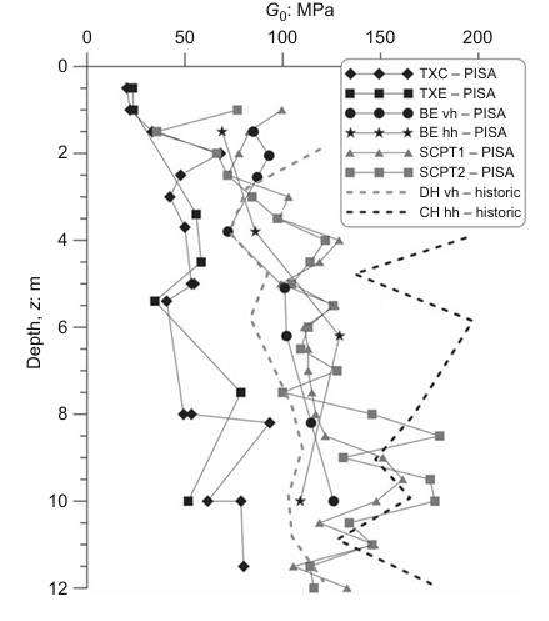
\includegraphics[width = 90mm]{Figures/figure1.pdf}
    \caption{Stiffness characteristics at Cowden \protect\citep{zdravkovic2020}}
    \label{fig:fig1.1}
\end{figure}


At the same time, with the increasing complexity and high-fidelity in geotechnical engineering problems, digital twin (DT) has gained popularity in handling abundant data and predict the structure's response in a more organized and accurate manner \citep{wang2021}. DT makes full use of data such as physical models, sensor updates and operating history, and integrates simulation processes to real-time reproduce the dynamics of a physical system in the virtual space. More importantly, the DT model cannot only describe the current state of the physical entity, but also predict the future state. However, state-of-the-art digital twins are still relying on considerable expertise and deployment resources \citep{kapteyn2021}, leading to an only one-off implementation and remaining limitation on providing adaptive digital models on unique offshore piles. Thus, scalable and unified models should be developed and incorporated into digital twin to enable a intelligent decision making.

Based on above, in practice, geotechnical engineers will benefit from having a site-specific digital model with a rapid analysis and intelligent decision making process.




















\section{Urgent need for a unified and scalable digital twins for piles}
The demand for efficiency, reliability, and safety continues to grow in offshore wind foundation constructions. Computational models are an invaluable tool
 for understanding complex pile behaviors; they can be used to simulate new pile designs, operating conditions, or control strategies to explore their bearing behavior. This reduces the need for costly experiments or field tests. However, insights gained from a computational model are contingent on the model being an accurate reflection of the underlying soil parameters. Moreover, real-world pile foundations are constantly changing and evolving throughout their lifecycle. Using a single static computational model that ignores these differences fundamentally limits the specificity,
 and thus the accuracy, of the model and any insights gained through its use.

 While the value proposition of digital twin has become widely appreciated in geotechnical engineering, the pile design process remains in a custom production phase. Current digital twin for offshore piles are still bespoken, relying on highly specialized implementations and thus requiring considerable resources and expertise to deploy and maintain. Therefore, it is necessary to move toward digital twins at scale by developing a rigorous and unified mathematical foundation. Meanwhile, based on the computational approaches and  probabilistic graphical model, scholars in aerospace engineering \citep{kapteyn2021} proposed a declarative and general digital twin model by leveraging techniques from computational science and engineering, autonomous systems, and machine learning. In this way, this mathematical foundation enables a promising application at scale in the offshore pile bearing response. 
 

 




\section{Objectives and outline}

The primary motivation of this thesis is to develop feasible and scalable digital twin model for offshore piles, based on the state-of-the-art techniques from aerospace engineering and computer science in order to enable predictive digital twin at scale. In particular, the specific goals of this thesis are:
\begin{itemize}
    \item Develop a methodology for back calculating soil parameters enabling to speed up the analysis and give in-time response for understanding the underlying uncertainties of soil parameters.
    \item Develop a unifying mathematical foundation for predictive digital twins for offshore piles in the form of a probabilistic graphical model.
\end{itemize}